\documentclass[14pt]{extarticle}
\usepackage{fontspec}
\usepackage{polyglossia}
\usepackage{amsmath}
\usepackage{amssymb}
\usepackage{xcolor}
\usepackage{fancyhdr}
\usepackage{graphicx}
\usepackage{listings}
\usepackage[most]{tcolorbox}
% \usepackage{setspace}
\usepackage{pifont}
\usepackage{enumitem}
\usepackage{titlesec}
\usepackage[bottom]{footmisc}
\usepackage{titling}
\usepackage{minted}
\usepackage{etoolbox}
\usepackage{array}
\usepackage{extsizes}
\usepackage{float}
\usepackage{booktabs}
\usepackage{hyperref}
\usepackage[onehalfspacing]{setspace}
\usepackage[a4paper, top=2.7cm, bottom=2.7cm, left=2.5cm, right=2.5cm, headheight=1.5cm, headsep=0.5cm]{geometry}
\usepackage{tikz}

\usetikzlibrary{automata, positioning, arrows.meta, arrows}

\newfontfamily\emoji{Segoe UI Emoji}

\pagestyle{fancy}

\setmainlanguage[numerals=western]{arabic}
\setotherlanguage{english}
% \newfontfamily\arabicfont[Script=Arabic]{Amiri}
\newfontfamily\arabicfont[Script=Arabic]{Calibri}
\newfontfamily\arabicfonttt[Script=Arabic]{Courier New}

\lstset{
  language=[Sharp]C,
  numbers=left,
  stepnumber=1,
  numbersep=8pt,
  frame=single,
  basicstyle=\ttfamily\small,
  keywordstyle=\color{blue},
  stringstyle=\color{red},
  commentstyle=\color{green!50!black}
}

\newif\ifdetailed
\ifdefined\setdetailed
  \setdetailed
\fi

\newif\ifwithsols
\ifdefined\setwithsols
  \setwithsols
\fi

% unified tcolorboxes for articles
\tcbset{colback=white, colframe=black, fonttitle=\bfseries, boxrule=0.8pt}
\newtcolorbox{boxDef}[1][]{colback=blue!5!white,colframe=blue!75!black,
  title={{\emoji📘} تعريف\ifx\\#1\\\else ~#1\fi :}}
\newtcolorbox{boxExercise}[1][]{colback=cyan!5!white,colframe=cyan!70!black,
  title={{\emoji🧩} تمرين\ifx\\#1\\\else ~#1\fi :}}
\newtcolorbox{boxExample}[1][]{colback=yellow!5!white,colframe=orange!90!black,
  title={{\emoji📝} مثال\ifx\\#1\\\else ~#1\fi :}}
\newtcolorbox{boxNote}[1][]{colback=gray!10!white,colframe=black,
  title={{\emoji✨} ملاحظة\ifx\\#1\\\else ~#1\fi :}}
\newtcolorbox{boxAttention}[1][]{colback=magenta!10!white,colframe=magenta!80!black,
  title={{\emoji🔔} تنبيه\ifx\\#1\\\else ~#1\fi :}}
\newtcolorbox{boxWarning}[1][]{colback=red!5!white,colframe=red!75!black,
  title={{\emoji⚡} ملاحظة هامة\ifx\\#1\\\else ~#1\fi :}}
\newtcolorbox{boxSolution}[1][]{colback=green!5!white,colframe=green!60!black,
  title={{\emoji✅} حل\ifx\\#1\\\else ~#1\fi :}}
\newtcolorbox{boxSymbol}[1][]{colback=purple!5!white,colframe=purple!70!black,
  title={{\emoji🔣} رمز\ifx\\#1\\\else ~#1\fi :}}
\newtcolorbox{boxHint}[1][]{colback=teal!5!white,colframe=teal!60!black,
  title={{\emoji💡} تلميح\ifx\\#1\\\else ~#1\fi :}}


\tcbset{simplecode/.style={ colback=gray!5, colframe=black!50, boxrule=0.4pt, arc=2pt, left=4pt,right=4pt,top=4pt,bottom=4pt}}
\newenvironment{boxCode}{\begin{tcolorbox}[simplecode]}{\end{tcolorbox}}

\newcolumntype{C}[1]{>{\centering\arraybackslash}p{#1}}

% redefine spaces after titles
\makeatletter
\renewcommand{\@maketitle}{%
  \begin{center}
    {\huge \bfseries \@title \par}%
    \vskip 0.2em % space between title and author
    {\large \@author \par}%
    % \vskip 0.2em % space between author and date
    % {\normalsize \@date \par}%
  \end{center}
}
\makeatother

\fancyhf{} % clear default
\fancypagestyle{plain}{
  \fancyhf{}
  \fancyhead[L]{مدرسة التسامح الشاملة}
  % \fancyhead[L]{
\includegraphics[height=1cm]{../../../images/logoTasamoh.png}}
  \fancyhead[R]{الأستاذ محمود اغبارية}
  \fancyfoot[C]{\thepage}
}

\fancyhead[L]{مدرسة التسامح الشاملة}
\fancyhead[R]{الأستاذ محمود اغبارية}
\fancyfoot[C]{\thepage}
% \date{\today}

\setcounter{tocdepth}{3} % only section subsection and subsubsection in TOC

\newcommand{\importpdfpage}[2]{%
    \thispagestyle{empty}
    \newgeometry{left=0cm,right=0cm,top=0cm,bottom=0cm}
    \includegraphics[page=#2,width=0.95\paperwidth,height=0.95\paperheight,keepaspectratio]{#1}
    \restoregeometry
}

\newcommand{\insertFullImg}[1]{%
    \noindent
    \makebox[\textwidth][c]{
        \includegraphics[width=0.9\paperwidth,keepaspectratio]{#1}%
    }%
}%

% ----------------------


% \begin{document}

% \maketitle

% % \clearpage  % start TOC on a new page
% % \renewcommand{\contentsname}{جدول المحتويات}
% % \tableofcontents
% % \clearpage

% \part*{part 1} % the * prevents numbering
% \section*{مقدمة}
% \subsection*{مثال رياضي}
% \subsubsection*{مثال فرعي}
% \paragraph*{ paragraph 1}
% \subparagraph*{sub paragraph 1}

% \ifdetailed
% \begin{english}
% \begin{minted}{csharp}
% // C# Example
% \end{minted}
% \end{english}
% \fi

% OLD WAY
% \ifdetailed
% \begin{english}
% \begin{lstlisting}
% // C# Example
% \end{lstlisting}
% \end{english}
% \fi

% % 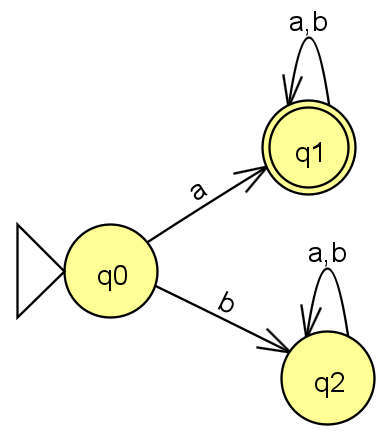
\includegraphics[width=0.2\textwidth]{../../../images/DFAs/ex1_q1.png}



% \vspace{3cm}
% \begin{flushleft}
% أرجو لكم وقتًا ممتعًا.

% الأستاذ محمود اغبارية.
% \end{flushleft}


% \end{document}


\ifwithsols
\title{حل وظيفة: الفئات والكائنات 1}
\else
\title{وظيفة: الفئات والكائنات 1}
\fi

\begin{document}

\maketitle
\thispagestyle{fancy}

\begin{enumerate}[itemsep=2em]

% ======================================================
% سؤال 1 - فئة BankAccount
% ======================================================
\item
سنبني فئة تمثل حسابًا بنكيًا.
\begin{enumerate}[itemsep=1em]
    \item أنشئ فئة باسم \textenglish{BankAccount} تحتوي على الحقول الخاصة (\textenglish{private}) التالية:
    \begin{itemize}[itemsep=1pt]
        \item \textenglish{string Owner} — اسم صاحب الحساب
        \item \textenglish{double Balance} — الرصيد الحالي
    \end{itemize}
    أضف عملية بنّاءة تستقبل اسم الصاحب ورصيدًا ابتدائيًا، مع التحقق من أنّ الرصيد غير سالب (إذا كان سالبًا تضعه 0).

    \item أضف عمليات \textenglish{GetOwner()} و \textenglish{GetBalance()}.

    \item أضف عملية \textenglish{void Deposit(double amount)} لإيداع مبلغ في الحساب.\\
    \textbf{شرط:} المبلغ يجب أن يكون أكبر من صفر.

    \item أضف عملية \textenglish{bool Withdraw(double amount)} لسحب مبلغ من الحساب.\\
    تعيد \textenglish{true} إذا نجحت العملية، و\textenglish{false} إذا كان الرصيد غير كافٍ أو المبلغ غير صالح.\\
    \textbf{شرط:} المبلغ أكبر من صفر والرصيد كافٍ.

    \item أضف عملية \textenglish{void Print()} تطبع اسم الصاحب والرصيد.

    \item في الدالة الرئيسية \textenglish{Main}، اكتب الأوامر التالية بالترتيب لاختبار الفئة:
    \begin{enumerate}[itemsep=1pt, label=(\roman*)]
        \item عرّف كائنًا يمثل حسابًا بنكيًا باسم \textenglish{"Ahmad"} وبرصيد ابتدائي قدره \textenglish{500.0}، ثم اطبعه باستخدام \textenglish{Print()}.
        \item قم بإيداع مبلغ \textenglish{200} في الحساب باستخدام الدالة \textenglish{Deposit()}، ثم اطبع بيانات الحساب مجددًا.
        \item حاول سحب مبلغ \textenglish{800} باستخدام الدالة \textenglish{Withdraw()}. احفظ القيمة التي تعيدها العملية في متغير واطبعها لمعرفة ما إذا نجحت العملية، ثم اطبع حالة الحساب للتأكد من عدم تغير الرصيد.
        \item حاول سحب مبلغ \textenglish{300} بالطريقة نفسها. اطبع القيمة التي تعيدها العملية، ثم اطبع بيانات الحساب لرؤية الرصيد الجديد بعد السحب.
    \end{enumerate}
\end{enumerate}

\ifwithsols
{\small
\begin{boxSolution}
\begin{english}
\begin{minted}{csharp}
class BankAccount
{
    private string Owner;
    private double Balance;

    public BankAccount(string owner, double balance)
    {
        this.Owner   = owner;
        if(balance < 0)
            this.Balance = 0;
        else
            this.Balance = balance;
    }

    public string GetOwner()   { return Owner;   }
    public double GetBalance() { return Balance; }

    public void Deposit(double amount)
    {
        if (amount > 0)
            Balance += amount;
    }

    public bool Withdraw(double amount)
    {
        if (amount <= 0 || amount > Balance)
            return false;
        Balance -= amount;
        return true;
    }

    public void Print()
    {
        Console.WriteLine($"Owner: {Owner} | Balance: {Balance}");
    }
}
\end{minted}
\end{english}
\end{boxSolution}
\begin{boxSolution}
\begin{english}
\begin{minted}{csharp}
public static void Main()
{
    BankAccount acc = new BankAccount("Ahmad", 500.0);
    acc.Print();

    acc.Deposit(200);
    acc.Print();

    bool ok1 = acc.Withdraw(800);
    Console.WriteLine("Withdraw 800: " + ok1);
    acc.Print();

    bool ok2 = acc.Withdraw(300);
    Console.WriteLine("Withdraw 300: " + ok2);
    acc.Print();
}
\end{minted}
\end{english}
\end{boxSolution}
}
\fi
\clearpage

% ======================================================
% سؤال 2 - فئة Product
% ======================================================
\item
سنبني فئة تمثل منتجًا في متجر.
\begin{enumerate}[itemsep=1em]
    \item أنشئ فئة باسم \textenglish{Product} تحتوي على الحقول الخاصة (\textenglish{private}) التالية:
    \begin{itemize}[itemsep=1pt]
        \item \textenglish{string Name} — اسم المنتج
        \item \textenglish{double Price} — السعر (يجب أن يكون أكبر من صفر)
        \item \textenglish{int Stock} — الكمية المتوفرة في المخزون
    \end{itemize}
    أضف عملية بنّاءة تستقبل الاسم والسعر والكمية، مع التحقق من أنّ السعر أكبر من صفر وإلا تضعه $0.01$، وأنّ الكمية غير سالبة وإلا تضعها 0.

    \item أضف عمليات الاسترجاع (Getters) لجميع الحقول.

    \item أضف عملية \textenglish{bool IsAvailable()} تعيد \textenglish{true} إذا كانت الكمية أكبر من صفر.

    \item أضف عملية \textenglish{bool Sell(int quantity)} لبيع كمية من المنتج.\\
    تعيد \textenglish{true} إذا نجحت (الكمية المطلوبة موجودة في المخزون)، وتُنقص \textenglish{Stock} بالكمية المباعة.\\
    تعيد \textenglish{false} إذا لم تكن الكمية متوفرة أو كانت المعطى غير صالح.

    \item أضف عملية \textenglish{double TotalValue()} تعيد إجمالي قيمة المنتج في المخزون \\ (\textenglish{Price * Stock}).

    \item أضف عملية \textenglish{void Print()} تطبع المنتج بالتنسيق التالي: \\
    \textenglish{Product: Pen | Price: 5.5 | Stock: 100} \\
    وإذا كان المخزون فارغًا، أضف \textenglish{" [Out of Stock]"} في النهاية.

    \item في الدالة الرئيسية \textenglish{Main}، قُم بكتابة الأوامر التالية بالترتيب لاختبار الفئة:
    \begin{enumerate}[itemsep=1pt, label=(\roman*)]
        \item عرّف كائنًا يمثل منتجًا باسم \textenglish{"Notebook"}، بسعر \textenglish{12.5}، وبكمية مخزون ابتدائية تبلغ 5 وحدات.
        \item استدعِ الدالة \textenglish{Print()} لطباعة تفاصيل المنتج الأولية.
        \item حاول بيع 3 وحدات من المنتج باستخدام الدالة \textenglish{Sell()}. احفظ النتيجة واطبعها للتأكد من نجاح العملية، ثم اطبع بيانات المنتج مجددًا لرؤية المخزون الجديد.
        \item حاول بيع 4 وحدات إضافية. اطبع نتيجة الدالة، ثم اطبع بيانات المنتج للتأكد من أن المخزون لم يتغير.
    \end{enumerate}
\end{enumerate}

\ifwithsols
{\small
\begin{boxSolution}
\begin{english}
\begin{minted}{csharp}
class Product
{
    private string Name;
    private double Price;
    private int Stock;

    public Product(string name, double price, int stock)
    {
        this.Name  = name;
        this.Price = (price > 0) ? price : 0.01;
        this.Stock = (stock >= 0) ? stock : 0;
    }

    public string GetName()  { return Name;  }
    public double GetPrice() { return Price; }
    public int    GetStock() { return Stock; }

    public bool IsAvailable()
    {
        return Stock > 0;
    }

    public bool Sell(int quantity)
    {
        if (quantity <= 0 || quantity > Stock)
            return false;
        Stock -= quantity;
        return true;
    }

    public double TotalValue()
    {
        return Price * Stock;
    }

    public void Print()
    {
        Console.Write($"Product: {Name} | Price: {Price} | Stock: {Stock}");
        if (!IsAvailable())
            Console.Write(" [Out of Stock]");
        Console.WriteLine();
    }
}
\end{minted}
\end{english}
\end{boxSolution}
\begin{boxSolution}
\begin{english}
\begin{minted}{csharp}
public static void Main()
{
    Product p = new Product("Notebook", 12.5, 5);
    p.Print();

    bool ok1 = p.Sell(3);
    Console.WriteLine("Sold 3: " + ok1);
    p.Print();

    bool ok2 = p.Sell(4);
    Console.WriteLine("Sold 4: " + ok2);
    p.Print();
}
\end{minted}
\end{english}
\end{boxSolution}
}
\fi

\end{enumerate}

\end{document}
